%%%%%%%%%%%%%%%%%%%%%%%%%%%%%%%%%%%%%%%%%
% University Assignment Title Page 
% LaTeX Template
% Version 1.0 (27/12/12)
%
% This template has been downloaded from:
% http://www.LaTeXTemplates.com
%
% Original author:
% WikiBooks (http://en.wikibooks.org/wiki/LaTeX/Title_Creation)
%
% License:
% CC BY-NC-SA 3.0 (http://creativecommons.org/licenses/by-nc-sa/3.0/)
% 
% Instructions for using this template:
% This title page is capable of being compiled as is. This is not useful for 
% including it in another document. To do this, you have two options: 
%
% 1) Copy/paste everything between \begin{document} and \end{document} 
% starting at \begin{titlepage} and paste this into another LaTeX file where you 
% want your title page.
% OR
% 2) Remove everything outside the \begin{titlepage} and \end{titlepage} and 
% move this file to the same directory as the LaTeX file you wish to add it to. 
% Then add \input{./title_page_1.tex} to your LaTeX file where you want your
% title page.
%
%%%%%%%%%%%%%%%%%%%%%%%%%%%%%%%%%%%%%%%%%
%\title{Title page with logo}
%----------------------------------------------------------------------------------------
%	PACKAGES AND OTHER DOCUMENT CONFIGURATIONS
%----------------------------------------------------------------------------------------

\documentclass[12pt]{article}
\usepackage[english]{babel}
\usepackage[utf8x]{inputenc}
\usepackage{amsmath}
\usepackage{graphicx}
\usepackage{caption}
\usepackage{subcaption}
\usepackage{hyperref}
\usepackage[colorinlistoftodos]{todonotes}
\usepackage{listings}
\usepackage{color}
\usepackage{float}
\usepackage{multirow}
\usepackage[normalem]{ulem}
\usepackage{adjustbox}
\usepackage[a4paper, total={6in, 8in}]{geometry}

\definecolor{dkgreen}{rgb}{0,0.6,0}
\definecolor{gray}{rgb}{0.5,0.5,0.5}
\definecolor{mauve}{rgb}{0.58,0,0.82}

\lstset{frame=tb,
  language=Java,
  aboveskip=3mm,
  belowskip=3mm,
  showstringspaces=false,
  columns=flexible,
  basicstyle={\small\ttfamily},
  numbers=none,
  numberstyle=\tiny\color{gray},
  keywordstyle=\color{blue},
  commentstyle=\color{dkgreen},
  stringstyle=\color{mauve},
  breaklines=true,
  breakatwhitespace=true,
  tabsize=3
}

\begin{document}

\begin{titlepage}

\newcommand{\HRule}{\rule{\linewidth}{0.5mm}} % Defines a new command for the horizontal lines, change thickness here

\center % Center everything on the page
 
%----------------------------------------------------------------------------------------
%	HEADING SECTIONS
%----------------------------------------------------------------------------------------

\textsc{\LARGE Sorbonnes Université - Sciences}\\[1.5cm] % Name of your university/college
\textsc{\Large Master ANDROIDE}\\[0.5cm] % Major heading such as course name
\textsc{\large Projet de Résolution de problèmes}\\[0.5cm] % Minor heading such as course title

%----------------------------------------------------------------------------------------
%	TITLE SECTION
%----------------------------------------------------------------------------------------

\HRule \\[0.4cm]
{ \large \bfseries Metaheuristiques pour la résolution du problème de l'arbre de Steiner de poids minimum}\\[0.4cm] % Title of your document
\HRule \\[1.5cm]
 
%----------------------------------------------------------------------------------------
%	AUTHOR SECTION
%----------------------------------------------------------------------------------------

\begin{minipage}{0.4\textwidth}
\begin{flushleft} \large
\emph{Author:}\\
Tristan \textsc{de Blauwe} % Your name
\end{flushleft}
\end{minipage}
~
\begin{minipage}{0.4\textwidth}
\begin{flushright} \large
\emph{Supervisor:} \\
Patrice \textsc{Perny} \\% Supervisor's Name
Nadjet \textsc{Bourdache}% Supervisor's Name
\end{flushright}
\end{minipage}\\[2cm]

% If you don't want a supervisor, uncomment the two lines below and remove the section above
%\Large \emph{Author:}\\
%John \textsc{Smith}\\[3cm] % Your name

%----------------------------------------------------------------------------------------
%	DATE SECTION
%----------------------------------------------------------------------------------------

\vfill % Fill the rest ofthe page with whitespace
{\small \today}\\[2cm] % Date, change the \today to a set date if you want to be precise

\end{titlepage}
%----------------------------------------------------------------------------------------

%----------------------------------------------------------------------------------------
%	TABLE OF CONTENTS	
%----------------------------------------------------------------------------------------
\newpage
\tableofcontents

%----------------------------------------------------------------------------------------
%	INTRODUCTION	
%----------------------------------------------------------------------------------------
\newpage
\section*{Introduction}
	\paragraph{}Ce rapport est un des documents attendus dans le cadre du projet RP (Résolution de problèmes). Ce document est accompagné du code-source et des différentes ressources utililsées pour mener à bien ce projet.
     L’objet du projet est de tester quelques métaheuristiques pour répondre au problème de l'arbre minimum de Steiner, en particulier de comparer les résultats obtenus par un algorithme génétique et une méthode de recherche locale.
     Vous trouverez donc dans ce document les choix, les réalisations et les tests accomplis durant ce projet.

	\paragraph{} Pour mettre en oeuvre ce projet, il a été choisi d'utiliser java, en utilisant la bibliothèque suivante: 
	
\url{http://www.i3s.unice.fr/~hogie/software/index.php}

	Dans un premier temps, nous décrirons les implémentations des parties clés des algorithmes. Puis les tests et les conclusions apportées.

%----------------------------------------------------------------------------------------
%	PARTIE I	
%----------------------------------------------------------------------------------------
\newpage
\section{Un simple algorithme génétique}

	\pararaph{}La première méthode mise en place pour résoudre le problème de Steiner est un algorithme génétique. Les sections suivantes
expliqueront les implémentations des différentes étapes.

	\subsection{Codage d'un individu}

		Le codage d'un individu suit les consignes données dans le sujet. Nous récupérons le graphe du problème initial. Pour chaque noeud non terminal de ce graphe, il est ajouté dans la
chaine. Au final, l'individu est codé selon un tableau de boolean. True signifie que le noeud est présent dans le graphe associé à ce codage.

		\begin{lstlisting}
		public boolean[] parseGraphToCoding(WeightedGraph base) {

			boolean[] coding = new boolean[base.getNumberOfVertices()-base.getNumberOfTerminals()];

			int i = 0;
			for(int id:base.getVertices().toIntArray()) {
				if(!base.isVertexTerminal(id)) {
					if(containsVertex(id)) 	{ coding[i] = true; }
					else 					{ coding[i] = false;}
					i++;
				}
			}
			return coding;
		}
		\end{lstlisting}

	\subsection{Evaluation d'un individu}

		L'évaluation d'un individu se fait avec la fonction suivante :

		\begin{lstlisting}
		public static int computeFitness(WeightedGraph g) {
			int fitness = 0;

			WeightedGraph mst 	= g.kruskal();

			if(mst.isConnected()) {
				fitness = mst.sumWeight();
			}else {
				int forestWeight    = mst.sumWeight();
				int M               = PENALITY;
				int nbVerticesMst   = mst.getNumberOfVertices();
				int nbEdgesMst      = mst.getNumberOfEdges();

				fitness = forestWeight + M * (nbVerticesMst - 1 - nbEdgesMst);
			}
			return fitness;
		}
		\end{lstlisting}

	\subsection{Opérateur de sélection et croissement}
		Comme opérateur de croissement, nous avons choisis d'utiliser un opérateur à un point, qui est implémenté  avec la fonction suivante :

		\begin{lstlisting}
		public static Individual[] crossover(Individual a, Individual b) {

			Individual[] childs = new Individual[2];
			childs[0] = new Individual(false);
			childs[1] = new Individual(false);

			int rnd = HandyTools.randInt(1, a.getGenes().length-1);	// Exclusion des bornes pour avoir un crossover significatif
			
			for(int i=0; i<a.getGenes().length; i++) {
				if(i<rnd) {
					childs[0].setGene(i, a.getGene(i));
					childs[1].setGene(i, b.getGene(i));
				}else {
					childs[0].setGene(i, b.getGene(i));
					childs[1].setGene(i, a.getGene(i));
				}
			}

			return childs;
		}
		\end{lstlisting}
		Aucun autre opérateur n'a été testé.

		Quant à la sélection des parents, nous utilisons la sélection par roulette :
		\begin{lstlisting}
		private int rouletteSelect() {
			int	leastFittest = getLeastFittest().getFitness();	
			int index;
			while (true) {
				index = HandyTools.randInt(0, getPopulationSize());
				if (HandyTools.randProb((1-getIndividual(index).getFitness() / leastFittest))) break;
			}
			return index;
		}
		\end{lstlisting}

		Cette méthode permet de sélectionner des individus, dont leur probabilité d'être tiré est proportionnelle à leur fitness.
Ce qui permet aux meilleurs d'être tiré plus souvent, mais de tout de même selectionner d'autres individus, dans le but de garder une diversité.
D'autres méthodes auraient pu être utilisé comme la sélection par tournoi, plus coûteuse. Cependant, cette méthode a pour avantage d'être très peu couteuse
tout en étant efficace. D'où ce choix.

	\subsection{Mutation}

		Pour la mutation, un individu dans une population a une certaine probabilité de muter (paramétrable) :
		\begin{lstlisting}
		for(int i=0; i<getPopulationSize(); i++) {
			if (HandyTools.randProb(SimpleGeneticAlgorithm.MUTATION_RATE)) { getIndividual(i).mutate();}
		}
		\end{lstlisting}

		Si c'est le cas, alors un de ces gènes va être modifié (inversion de bit). Pour accélerer la vitesse d'execution de notre programme
, nous mettons en cache la valeur de qualité de l'individu. Il faut donc relancer le calcul de qualité après mutation (si cette valeur est
à nouveau demandé, sinon on ne la calcule pas). Au cours de nos tests, nous avons obtenu de meilleurs résultats en mettant le taux de mutation à 0.4.
En le mettant plus bas, notre algorithme convergait plus lentement vers l'optimal.

		\begin{lstlisting}
		public void mutate() {
			int mutationIndex = HandyTools.randInt(0, genes.length);
			genes[mutationIndex] = !genes[mutationIndex];
			fitness = 0;	// Pour relancer le calcul de fitness
		}
		\end{lstlisting}

	\subsection{Replacement et nouvelle génération}

	Dans notre impléntation, la nouvelle génération peut-être générée de deux manières différentes. Soit, elle est composée uniquement des
enfants issus des croisements, ou alors, composée des meilleurs individus des deux générations (Parents et enfants).
Ici, nous prenons la moitié des meilleurs des enfants et la moitié des meilleurs des enfants :

		\begin{lstlisting}
		switch(SimpleGeneticAlgorithm.replacementStrat) {
			case ELITIST:
				Individual[] fittestFromParents 	= getFittest(getPopulationSize()/2);
				Individual[] fittestFromChildrens 	= childrens.getFittest(getPopulationSize()/2);
				for(int i=0; i<getPopulationSize()/2; i++) {
					newGen.saveIndividual(fittestFromParents[i]);
					newGen.saveIndividual(fittestFromChildrens[i]);
				}
				break;

			default:
				newGen = childrens;
				break;
		}
		\end{lstlisting}

	\paragraph{}Au début, nous faisions en sorte que le meilleur individu soit gardé intacte dans la nouvelle génération. Nous empêchions donc qu'il
mute. Cependant, ce choix nous posait des problèmes lors de la résolution de certaines instances, où nous restions bloqué dans un minimum local.
Il a donc été décidé de le laisser muter si besoin est, ce qui a permis d'obtenir de meilleurs résultats par la suite.

	\paragraph{} Selon nos tests et l'implémentation de notre solution, il ne semble pas y avoir de majeure différence entres les deux méthodes de remplacement:

	\begin{figure}[H]
	\centering
		\begin{minipage}{.5\textwidth}
		  \centering
		  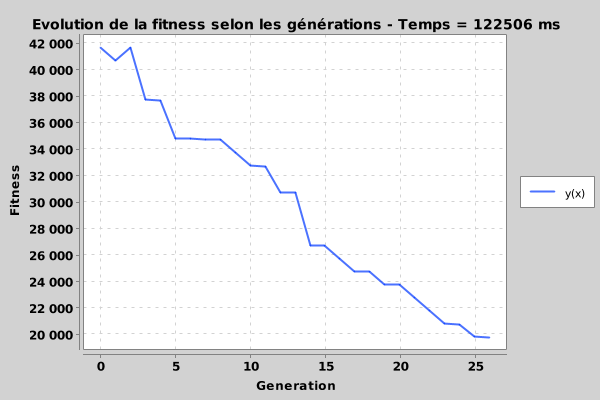
\includegraphics[width=1\linewidth]{images/OnlyBest}
		  \captionof{figure}{Elitiste}
		  \label{fig:test1}
		\end{minipage}%
		\begin{minipage}{.5\textwidth}
		  \centering
		  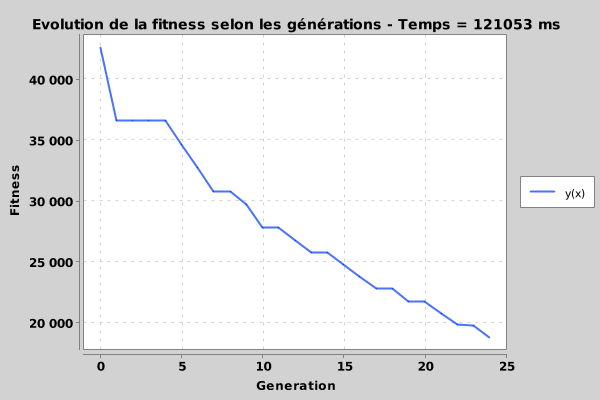
\includegraphics[width=1\linewidth]{images/OnlyChildrens}
		  \captionof{figure}{Genérationnelle}
		  \label{fig:test2}
		\end{minipage}
	\end{figure}

	Quant au nombre de génération maximale, nous avons autorisé au maximum 2000 générations. Pour les petites instances, la solution est en générale trouvée avant. Et pour les grosses instances, ce nombre est trop grand pour
être atteint avec un timeout faible. Il s'agit donc surtout de permettre de trouver la meilleure solution possible, si l'instance se déroule rapidement.	
	\subsection{Population initiale}

	Une des méthodes pour générer la population initiale, est de tout simplement générer des individus aléatoirement :

		\begin{lstlisting}
		public Individual(boolean generate) {
			fitness = 0;
			genes 	= new boolean[Bridge.getGenesLength()];
			
			if(generate) {
				double p =  HandyTools.randDouble(SimpleGeneticAlgorithm.TRUE_PROBABILITY_MIN, SimpleGeneticAlgorithm.TRUE_PROBABILITY_MAX);
				for(int i=0; i<genes.length; i++) {
					if(HandyTools.randProb(p)) { genes[i] = true; }
				}
			}
		}
		\end{lstlisting}

	Chaque individu a une probabilité aléatoire p qui détermine la probabilité qu'un gène soit à 1 ou 0. Le fait d'avoir une probabilité p
différente pour chaque individu permet d'améliorer la diversité.

	Nous avons décidé d'utiliser une population de taille 50. Ce paramètre permet d'obtenir un bon compromis entre efficacité et temps de calcul, même si
pour les plus grosses instances, il est préférable de baisser jusqu'à 30 par exemple.

	\paragraph{}Cependant, avec une population aléatoire, cette méthode donne de mauvaise résultats pour les grosses instances. Dans la prochaine partie, nous allons vous montrer les implémentations
des méthodes permettant d'améliorer la population initiale.
    
%----------------------------------------------------------------------------------------
%	PARTIE II
%----------------------------------------------------------------------------------------
\newpage
\section{Amélioration de la population avec heuristiques de construction}

	Cette partie décrit l'implémentation des deux nouvelles heuristiques, l'heuristique du plus court chemin et l'heuristique de l'arbre
couvrant minimum, ainsi que les nouvelles stratégies de génération de la population initiale.

	\subsection{Heuristique du plus court chemin}

		Voici l'implémentation de cette heuristique :

		\begin{lstlisting}
		public WeightedGraph generateShortestPathGraphHeuristic(boolean randomize) {

			NumericalProperty weights = this.getWeightsProperty();
			if(randomize) { weights = getRandomizedWeights(); }

			int[] terminalVertices = this.terminalVertices.stream().mapToInt(Integer::intValue).toArray();
			DistanceMatrix 	distMatrix = new StackBasedBellmanFordWeightedMatrixAlgorithm(weights).compute(this);

			WeightedGraph g1 = new WeightedGraph();
			int edge = 0;
			for (int i = 0; i < terminalVertices.length; i++) {
				for (int j = i + 1; j < terminalVertices.length; j++) {
					if(!g1.containsVertex(terminalVertices[i])) { g1.addVertex(terminalVertices[i]); }
					if(!g1.containsVertex(terminalVertices[j])) { g1.addVertex(terminalVertices[j]); }
					g1.addEdge(edge, terminalVertices[i], terminalVertices[j] , distMatrix.get(terminalVertices[i], terminalVertices[j]));
					edge++;
				}
			}

			WeightedGraph g2 = g1.kruskal();

			PredecessorMatrix predMatrix = new WeightedPredecessorMatrixAlgorithm(weights).compute(this);
			WeightedGraph g3 = new WeightedGraph();
			for(int edgeId:g2.getEdges().toIntArray()) {
				int 	source 		= g2.getOneVertex(edgeId);
				int 	destination = g2.getTheOtherVertex(edgeId, source);
				if(!g3.containsVertex(source)) { g3.addVertex(source); }
				if(!g3.containsVertex(destination)) { g3.addVertex(destination); }

				int 	formerPred 	= destination;
				int 	pred 		= predMatrix.getPredecessor(source, destination);

				while(formerPred != source) {
					edgeId = getEdgesConnecting(pred, formerPred).toIntArray()[0];
					if(!g3.containsVertex(pred)) { g3.addVertex(pred); }
					if(!g3.containsEdge(edgeId)) { g3.addEdge(edgeId, pred, formerPred, getEdgeWeight(edgeId)); }
					formerPred = pred;
					pred = predMatrix.getPredecessor(source, pred);
				}
			}

			WeightedGraph g4 = g3.kruskal();
			for(int vertex:g4.getVertices().toIntArray()) {
				if(isVertexTerminal(vertex)) {
					g4.addTerminalVertex(vertex);
				}else {
					if(g4.getVertexDegree(vertex) <= 1) {
						g4.removeVertex(vertex);
					}
				}
			}
			return g4;	// G5 is built during the for loop
		}
		\end{lstlisting}

	\subsection{Heuristique de l'arbre couvrant minimum}

		Voici l'implémentation de cette heuristique :

		\begin{lstlisting}
		public WeightedGraph generateMinimalSpanningTreeGraphHeuristic(boolean randomize) {
			NumericalProperty weights = this.getWeightsProperty();
			if(randomize) { weights = getRandomizedWeights(); }

			WeightedGraph g1 = WeightedGraph.kruskal(this, weights);

			boolean elimination = true;
			while(elimination) {
				elimination = false;
				for(int vertex:g1.getVertices().toIntArray()) {
					if(!isVertexTerminal(vertex) && (g1.getVertexDegree(vertex) <= 1)) {
							g1.removeVertex(vertex);
							elimination = true;
					}
				}
				if(elimination) { g1 = g1.kruskal(); }	
			}

			for(int vertex:terminalVertices) {
				g1.addTerminalVertex(vertex);
			}
			return g1;
		}
		\end{lstlisting}

	\subsection{Randomisation des heuristiques de construction}

	Les graphes étant parfois très volumineux, modifier le coût des arêtes était très coûteux, si le graphe devait être copié. Heureusement,
la bibliothèque utilisée permet de dupliquer une propriété contenant le poids des arêtes. Il est donc possible d'avoir un même graphe, mais
plusieurs propriétés de poids, donc sans duplication de graphe. D'où le code suivant permettant de randomiser le poids des arêtes :
		\begin{lstlisting}
		public NumericalProperty getRandomizedWeights() {
			NumericalProperty _weights = new NumericalProperty("weigths",8,1);	

			double variation = HandyTools.randDouble(SimpleGeneticAlgorithm.WEIGHT_RANDOM_OFFSET_MIN, SimpleGeneticAlgorithm.WEIGHT_RANDOM_OFFSET_MAX);
			for (int edge : getEdges().toIntArray())
			{
				float weight = weights.getValue(edge);
				if(HandyTools.randInt(0, 2)==1) {
					weight += weight * variation;
				}else {
					weight -= weight * variation;
				}
				_weights.setValue(edge, (int) Math.floor(weight));
			}
			return _weights;
		}
		\end{lstlisting}

	Ici, les poids subissent une variation aléatoire entre deux bornes réglables.

	\paragraph{}Grâce à ces nouvelles heuristiques, il est désormais possible de générer une meilleure population initiale. Notre programme
dispose de trois stratégies de générations :
	\begin{description}
	\item[RANDOM]	- Individus générés aléatoirement
	\item[IMPROVED] - Individus générés selon les deux heuristiques + aléatoire (1/3 de chaque) ! Très coûteux pour générer la pop° initiale !
	\item[MINIMAL]  - Individus générés selon les deux heuristiques + aléatoire (Pour les deux heuristiques, elles utilisent le taux spécifié, le reste est aléatoire)
	\end{description}

	Si nous avons implémenté la stratégie mininale, c'est parce que la génération des individus selon les deux heuristiques est très coûteuse sur les très grosse instance. Donc cette
stratégie n'en génère que quelques-uns (réglable selon des paramètres), afin d'obtenir un temps d'éxécution raisonnable, tous en gardant une bonne population initiale.
    
%----------------------------------------------------------------------------------------
%	PARTIE III
%----------------------------------------------------------------------------------------
\newpage
\section{Recherche Locale}

	Pour la mise en place de la recherche locale, nous détaillerons les étapes clés de l'algorithme.

	\subsection{Génération d'une solution}

		\paragraph{} Notre programme génère une solution selon 4 stratégies différentes:

	\begin{description}
	\item[RANDOM]	- Solution générée aléatoirement
	\item[ALL]		- Solution générée selon les deux heuristiques + aléatoire (1/3 de chaque)
	\item[MSP]		- Solution générée selon l'heuristique de l'arbre couvrant de poids minimum
	\item[SP]		- Solution générée selon l'heuristique du plus court chemin
	\end{description}

		\paragraph{}

	En utilisant les deux heuristiques, aucun mouvement n'est accomplie, puisqu'avec les règles d'ignorement aucun voisin n'est possible candidat. C'est pour cela
que la stratégie ALL a été mise en place, et qu'un paramètre pour déterminer si oui ou non les règles d'ignorement sont utilisées.

	La fonction responsable de la génération d'une solution est la suivante :
		\begin{lstlisting}
		private void generateSolution() {
			generateNewSolution = false;
			WeightedGraph g;

			boolean randomize = (this.movementCount == 0 ) ? false : true; // La première tentative n'est pas randomisée
			switch(GENERATION) {
				case ALL:
					int choice = HandyTools.randInt(0, 3);
					if(choice==0) {
						g = (base.generateMinimalSpanningTreeGraphHeuristic(randomize));
						setCurrentSolution(g, 0);
					}else if(choice==1) {
						g = (base.generateShortestPathGraphHeuristic(randomize));
						setCurrentSolution(g, 0);
					}else if(choice==2) {
						boolean[] genes = new boolean[Bridge.getGenesLength()];
						double p =  HandyTools.randDouble(0, 1);
						for(int i=0; i<Bridge.getGenesLength(); i++) {
							if(HandyTools.randProb(p)) { genes[i] = true; }
						}
						g = new WeightedGraph(base, genes);
						setCurrentSolution(g, 0);
					}
					break;
				
				case RANDOM:
					boolean[] genes = new boolean[Bridge.getGenesLength()];
					double p =  HandyTools.randDouble(0, 1);
					for(int i=0; i<Bridge.getGenesLength(); i++) {
						if(HandyTools.randProb(p)) { genes[i] = true; }
					}
					g = new WeightedGraph(base, genes);
					setCurrentSolution(g, 0);
					break;

				case MSP:
					g = (base.generateMinimalSpanningTreeGraphHeuristic(randomize));
					setCurrentSolution(g, 0);
					break;

				case SP:
					g = (base.generateShortestPathGraphHeuristic(randomize));
					setCurrentSolution(g, 0);
					break;
			}
		}
		\end{lstlisting}

	\paragraph{} Notre algorithme de recherche locale continue de fonctionner, tant que la solution optimale n'a pas été trouvé ou tant qu'il reste du temps. Si une solution non optimale est trouvé, on relance l'algorithme
avec une autre solution.

		Voici la majeure partie de la boucle principale de notre algorithme :
		\begin{lstlisting}
		while( (System.nanoTime() - startTime)/1000000 < TIMEOUT*60000 && solValue != opt ) {

			if(generateNewSolution) { 
				this.movementCount = 0;
				this.researchCount += 1;
				generateSolution(); 
			}

			TreeMap<Integer, WeightedGraph> candidates = getCandidates();
			if(!candidates.isEmpty()) {
				int value = candidates.firstKey();
				if(candidates.firstKey() < solValue) {
					setCurrentSolution(candidates.get(value), value);
					this.movementCount +=1;
				}else {
					generateNewSolution = true;
				}
			}else {
				generateNewSolution = true;
			
		\end{lstlisting}

	\paragraph{} Pour récupérer les candidats possibles, c'est-à-dire les mouvements possibles depuis la solution courante, nous avons simplement implémenté les consignes du sujet. En
voici l'implémentation :

		\begin{lstlisting}
		private TreeMap<Integer, WeightedGraph> getCandidates() {
			TreeMap<Integer, WeightedGraph> candidates = new TreeMap<Integer, WeightedGraph>();
			boolean saveCandidate = false;

			for(int vertex:base.getVertices()) {
				if(!base.isVertexTerminal(vertex)) {
					WeightedGraph candidate = new WeightedGraph(currentSol);
					if(currentSol.containsVertex(vertex)) {
						candidate.removeVertex(vertex);
						if(candidate.isConnected() || !LocalResearchAlgorithm.LIMIT_NEIGHBOURS) {
							saveCandidate = true;
						}
					}else {
						candidate.addVertex(vertex);
						if(candidate.getVertexDegree(vertex) > 1 || !LocalResearchAlgorithm.LIMIT_NEIGHBOURS) {
							saveCandidate = true;
						}
					}
					if(saveCandidate) {
						candidate = candidate.kruskal();
						candidates.put(Bridge.computeFitness(candidate), candidate);
					}
				}
			}
			return candidates;
		}
		\end{lstlisting}
%----------------------------------------------------------------------------------------
%	PARTIE IV
%----------------------------------------------------------------------------------------
\newpage
\section{Instances et évaluation}

	Désormais, dans cette section, nous allons vous décrire les résultats de nos algorithmes avec différents paramètres. Vu le temps limité et les possibilités très nombreuses, nous n'avons pas pu accomplir toutes les
comparaisons possibles selon nos différents paramètres. Nous avons donc décidé de comparer les 4 algorithmes suivants sur un nombre raisonnable d'instances :

	\begin{description}
	\item[SGA - Random  ]	- Algorithme génétique avec population initiale générée aléatoirement
	\item[SGA - Improved]	- Algorithme génétique avec population initiale générée avec la stratégie Improved (2 heuristiques + random)
	\item[LRA - Ignore  ]	- Algorithme de recherche locale avec les règles d'ignorement
	\item[LRA - No ignore]	- Algorithme de recherche locale sans les règles d'ignorenent
	\end{description}

	Pour les instances B à C, le timeout était fixé à 1 minutes, pour D+ à 2 minutes. Cependant, vous remarquerez que certaines instances dépasse le timeout. Cela concerne uniquement la recherche locale, puisque nous lui laissons 
le temps de finir au moins une solution avant de vérifier le timeout.

	Voici les paramètres de l'algorithme génétique utilisés lors des tests:

		\begin{lstlisting}
	public static double 	MUTATION_RATE 				= 0.4; 		// Probabilite qu'un individu mute
	public static double 	TRUE_PROBABILITY_MIN 		= 0.20; 	// Valeur min de la probabilite qu'un chromosome soit a 1 (lors de la creation d'un nouvel individu)
	public static double 	TRUE_PROBABILITY_MAX 		= 0.50; 	// Valeur max de la probabilite qu'un chromosome soit a 1 (lors de la creation d'un nouvel individu)
	public static double 	WEIGHT_RANDOM_OFFSET_MIN 	= 0.05; 	// Variation minimale d'un poids de sa valeur initial 
	public static double 	WEIGHT_RANDOM_OFFSET_MAX 	= 0.40; 	// Variation maximale d'un poids  de sa valeur initial 
	public static int 	INITIAL_POP_SIZE 			= 50; 		// Taille de la population (Doit etre paire (par simplicite))
	public static int 	MAX_GENERATIONS 			= 2000; 	// Nombre maximum de generation a produire
	public static int 	MAX_IND_FROM_SP_HEURISTIC 	= 3; 		// Nombre maximum d'individus a produire selon l'heuristique du plus court chemins
	public static int 	MAX_IND_FROM_MSP_HEURISTIC 	= 3; 		// Nombre maximum d'individus a produire selon l'heuristique de l'arbre couvrant de poids minimum

	public static ReplacementStrategy replacementStrat 	= ReplacementStrategy.ELITIST; 	// Selon quelle stratégie, l'algorithme doit-il former la nouvelle génération
	\end{lstlisting}

	Voici les paramètres de l'algorithme recherche locale utilisés lors des tests:

		\begin{lstlisting}
	public static final double 	WEIGHT_RANDOM_OFFSET_MIN 	= 0.05; 	// Variation minimale d'un poids de sa valeur initial 
	public static final double 	WEIGHT_RANDOM_OFFSET_MAX 	= 0.40; 	// Variation maximale d'un poids  de sa valeur initial 

	public static final solutionGeneration 	GENERATION 		= solutionGeneration.ALL; 	// Type de generation pour les solutions
	\end{lstlisting}

	Vous trouverez dans les pages suivantes les résultats de ces tests. Dans le dossier ./Charts ,disponible dans le livrable, vous trouverez aussi les graphes associés à ces tests, montrant l'évolution de la fitness au fil des générations, pour l'algorithme 
génétique, au fil des recherches (et non des mouvements) pour la recherche locale. Nous en avons inclus quelqu'uns dans la suite de ce document

	\begin{figure}[H]
	\centering
		\begin{minipage}{.5\textwidth}
		  \centering
		  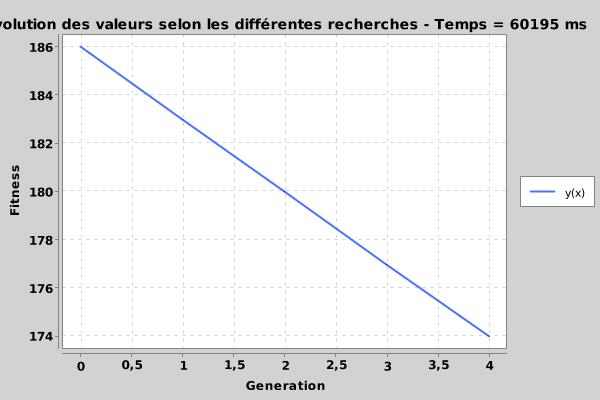
\includegraphics[width=1\linewidth]{images/c16 - LRA with ignore.jpg}
		  \captionof{figure}{c16 - LRA with ignore}
		\end{minipage}%
		\begin{minipage}{.5\textwidth}
		  \centering
		  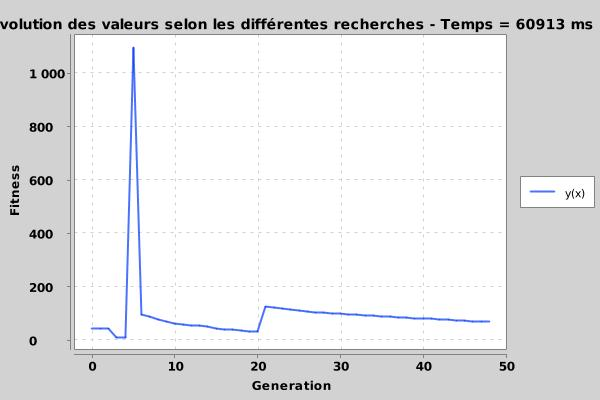
\includegraphics[width=1\linewidth]{images/c16 - LRA without ignore.jpg}
		  \captionof{figure}{c16 - LRA without ignore}
		\end{minipage}
	\end{figure}

	\begin{figure}[H]
	\centering
		\begin{minipage}{.5\textwidth}
		  \centering
		  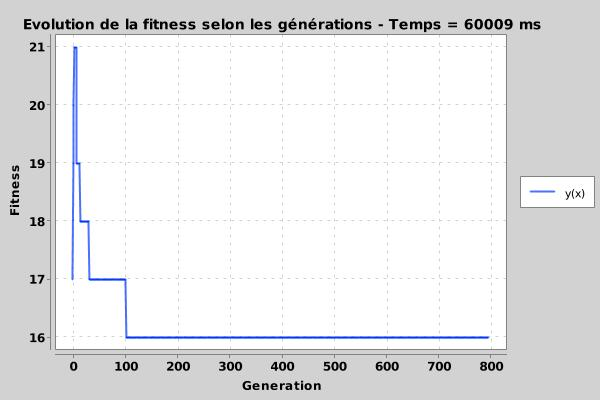
\includegraphics[width=1\linewidth]{images/c16 - SGA with improved pop gen.jpg}
		  \captionof{figure}{c16 - SGA with improved pop gen}
		\end{minipage}%
		\begin{minipage}{.5\textwidth}
		  \centering
		  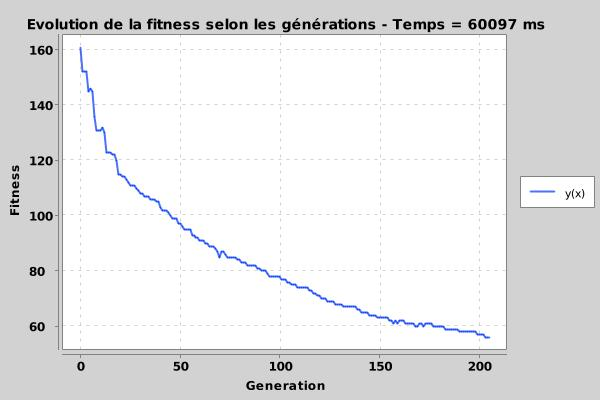
\includegraphics[width=1\linewidth]{images/c16 - SGA with random pop gen.jpg}
		  \captionof{figure}{c16 - SGA with random pop gen}
		\end{minipage}
	\end{figure}

	\paragraph{} Vous pouvez remarquer pour les deux algorithmes génétiques, qu'avec la population initiale améliorée, la convergence est très rapide. Dès les premières
générations, la solution est très proche de l'optimal. Quant à la population aléatoire, elle tend progressivement vers l'optimal. Les deux n'ont pas atteint l'optimal, puisque ils ont tous les deux timeout.
Pour le SGA avec la population améliorée, on peut voir qu'il est resté bloqué dans un minimum local.
	Enfin, comparé à l'algorithme génétique, la recherche locale n'a pas réussi à trouver un bonne solution comparé, pour le même temps alloué.

\begin{table}[]
\caption{Tableaux de comparaison des différents algorithmes - A à C}
\begin{adjustbox}{angle=90}
\resizebox{\textheight}{!}{
\begin{tabular}{|c|c|l|l|l|l|l|l|l|l|l|l|l|l|}
\hline
\multirow{2}{*}{{\ul \textbf{instance}}} & \multirow{2}{*}{{\ul \textbf{Optimal}}} & \multicolumn{3}{c|}{{\ul \textbf{SGA - Random}}} & \multicolumn{3}{c|}{{\ul \textbf{SGA - Improved}}} & \multicolumn{3}{c|}{{\ul \textbf{LRA - w/ ignore}}} & \multicolumn{3}{c|}{{\ul \textbf{LRA - w/o ignore}}} \\ \cline{3-14} &  & \textit{Best Value} & \textit{ecart} & \textit{Time} & \textit{Best Value} & \textit{ecart} & \textit{Time} & \textit{Best Value} & \textit{ecart} & \textit{Time} & \textit{Best value} & \textit{ecart} & \textit{Time} \\ \hline

\multicolumn{1}{|l|}{b1} & \multicolumn{1}{l|}{82} &82 & ,00\% & 1137 ms  & 82 & ,00\% & 194 ms  & 82 & ,00\% & 14 ms  & 82 & ,00\% & 1653 ms \\ \hline
\multicolumn{1}{|l|}{b2} & \multicolumn{1}{l|}{83} &83 & ,00\% & 948 ms  & 83 & ,00\% & 155 ms  & 86 & 3,61\% & 60029 ms  & 86 & 3,61\% & 60022 ms \\ \hline
\multicolumn{1}{|l|}{b3} & \multicolumn{1}{l|}{138} &138 & ,00\% & 853 ms  & 138 & ,00\% & 239 ms  & 138 & ,00\% & 3622 ms  & 138 & ,00\% & 39885 ms \\ \hline
\multicolumn{1}{|l|}{b4} & \multicolumn{1}{l|}{59} &63 & 6,78\% & 22059 ms  & 59 & ,00\% & 116 ms  & 59 & ,00\% & 7 ms  & 59 & ,00\% & 265 ms \\ \hline
\multicolumn{1}{|l|}{b5} & \multicolumn{1}{l|}{61} &61 & ,00\% & 903 ms  & 61 & ,00\% & 133 ms  & 62 & 1,64\% & 60026 ms  & 62 & 1,64\% & 60067 ms \\ \hline
\multicolumn{1}{|l|}{b6} & \multicolumn{1}{l|}{122} &124 & 1,64\% & 60007 ms  & 122 & ,00\% & 218 ms  & 122 & ,00\% & 53363 ms  & 124 & 1,64\% & 60004 ms \\ \hline
\multicolumn{1}{|l|}{b7} & \multicolumn{1}{l|}{111} &111 & ,00\% & 3403 ms  & 111 & ,00\% & 215 ms  & 111 & ,00\% & 0 ms  & 111 & ,00\% & 0 ms \\ \hline
\multicolumn{1}{|l|}{b8} & \multicolumn{1}{l|}{104} &107 & 2,88\% & 60033 ms  & 104 & ,00\% & 260 ms  & 104 & ,00\% & 13 ms  & 104 & ,00\% & 0 ms \\ \hline
\multicolumn{1}{|l|}{b9} & \multicolumn{1}{l|}{220} &220 & ,00\% & 2097 ms  & 220 & ,00\% & 437 ms  & 220 & ,00\% & 0 ms  & 220 & ,00\% & 328 ms \\ \hline
\multicolumn{1}{|l|}{b10} & \multicolumn{1}{l|}{86} &86 & ,00\% & 39324 ms  & 86 & ,00\% & 731 ms  & 94 & 9,30\% & 60102 ms  & 94 & 9,30\% & 60020 ms \\ \hline
\multicolumn{1}{|l|}{b11} & \multicolumn{1}{l|}{88} &89 & 1,14\% & 55839 ms  & 88 & ,00\% & 797 ms  & 90 & 2,27\% & 60094 ms  & 90 & 2,27\% & 60111 ms \\ \hline
\multicolumn{1}{|l|}{b12} & \multicolumn{1}{l|}{174} &174 & ,00\% & 2536 ms  & 174 & ,00\% & 725 ms  & 174 & ,00\% & 43 ms  & 174 & ,00\% & 0 ms \\ \hline
\multicolumn{1}{|l|}{b13} & \multicolumn{1}{l|}{165} &168 & 1,82\% & 60045 ms  & 170 & 3,03\% & 60020 ms  & 175 & 6,06\% & 60061 ms  & 175 & 6,06\% & 60009 ms \\ \hline
\multicolumn{1}{|l|}{b14} & \multicolumn{1}{l|}{235} &1228 & 422,55\% & 60008 ms  & 236 & ,43\% & 60067 ms  & 237 & ,85\% & 60146 ms  & 237 & ,85\% & 60044 ms \\ \hline
\multicolumn{1}{|l|}{b15} & \multicolumn{1}{l|}{318} &320 & ,63\% & 60012 ms  & 318 & ,00\% & 791 ms  & 323 & 1,57\% & 60024 ms  & 323 & 1,57\% & 60030 ms \\ \hline
\multicolumn{1}{|l|}{b16} & \multicolumn{1}{l|}{127} &132 & 3,94\% & 60046 ms  & 127 & ,00\% & 7197 ms  & 137 & 7,87\% & 60091 ms  & 137 & 7,87\% & 60641 ms \\ \hline
\multicolumn{1}{|l|}{b17} & \multicolumn{1}{l|}{131} &131 & ,00\% & 12686 ms  & 131 & ,00\% & 712 ms  & 134 & 2,29\% & 60049 ms  & 134 & 2,29\% & 60245 ms \\ \hline
\multicolumn{1}{|l|}{b18} & \multicolumn{1}{l|}{248} &221 & 10,89\% & 60073 ms  & 218 & 12,10\% & 60043 ms  & 224 & 9,68\% & 4249 ms  & 224 & 9,68\% & 30219 ms \\ \hline
\multicolumn{1}{|l|}{c1} & \multicolumn{1}{l|}{85} &23037 & 27002,35\% & 61002 ms  & 86 & 1,18\% & 45066 ms  & 88 & 3,53\% & 145884 ms  & 118 & 38,82\% & 71807 ms \\ \hline
\multicolumn{1}{|l|}{c2} & \multicolumn{1}{l|}{144} &2151 & 1393,75\% & 60034 ms  & 144 & ,00\% & 4556 ms  & 144 & ,00\% & 0 ms  & 8008 & 5461,11\% & 72027 ms \\ \hline
\multicolumn{1}{|l|}{c3} & \multicolumn{1}{l|}{754} &33201 & 4303,32\% & 60877 ms  & 766 & 1,59\% & 60196 ms  & 780 & 3,45\% & 127844 ms  & 867 & 14,99\% & 173718 ms \\ \hline
\multicolumn{1}{|l|}{c4} & \multicolumn{1}{l|}{1079} &33460 & 3001,02\% & 62023 ms  & 1103 & 2,22\% & 60355 ms  & 1112 & 3,06\% & 154989 ms  & 62643 & 5705,65\% & 76317 ms \\ \hline
\multicolumn{1}{|l|}{c5} & \multicolumn{1}{l|}{1579} &24798 & 1470,49\% & 62271 ms  & 1584 & ,32\% & 60349 ms  & 1604 & 1,58\% & 60083 ms  & 55495 & 3414,57\% & 79271 ms \\ \hline
\multicolumn{1}{|l|}{c6} & \multicolumn{1}{l|}{55} &6118 & 11023,64\% & 61361 ms  & 60 & 9,09\% & 29453 ms  & 60 & 9,09\% & 130516 ms  & 60 & 9,09\% & 60447 ms \\ \hline
\multicolumn{1}{|l|}{c7} & \multicolumn{1}{l|}{102} &4215 & 4032,35\% & 60009 ms  & 103 & ,98\% & 60013 ms  & 115 & 12,75\% & 164988 ms  & 115 & 12,75\% & 127043 ms \\ \hline
\multicolumn{1}{|l|}{c8} & \multicolumn{1}{l|}{509} &8269 & 1524,56\% & 61491 ms  & 518 & 1,77\% & 60094 ms  & 531 & 4,32\% & 60006 ms  & 43590 & 8463,85\% & 64503 ms \\ \hline
\multicolumn{1}{|l|}{c9} & \multicolumn{1}{l|}{707} &5369 & 659,41\% & 60169 ms  & 728 & 2,97\% & 60911 ms  & 728 & 2,97\% & 121344 ms  & 3548 & 401,84\% & 116790 ms \\ \hline
\multicolumn{1}{|l|}{c10} & \multicolumn{1}{l|}{1093} &5471 & 400,55\% & 60354 ms  & 1105 & 1,10\% & 60538 ms  & 1122 & 2,65\% & 82573 ms  & 1662 & 52,06\% & 80622 ms \\ \hline
\multicolumn{1}{|l|}{c11} & \multicolumn{1}{l|}{32} &543 & 1596,88\% & 60646 ms  & 38 & 18,75\% & 58235 ms  & 37 & 15,62\% & 105634 ms  & 764 & 2287,50\% & 112001 ms \\ \hline
\multicolumn{1}{|l|}{c12} & \multicolumn{1}{l|}{46} &520 & 1030,43\% & 61661 ms  & 46 & ,00\% & 15598 ms  & 48 & 4,35\% & 158164 ms  & 48 & 4,35\% & 137236 ms \\ \hline
\multicolumn{1}{|l|}{c13} & \multicolumn{1}{l|}{258} &595 & 130,62\% & 61665 ms  & 279 & 8,14\% & 60234 ms  & 788 & 205,43\% & 83211 ms  & 866 & 235,66\% & 203428 ms \\ \hline
\multicolumn{1}{|l|}{c14} & \multicolumn{1}{l|}{323} &593 & 83,59\% & 62126 ms  & 337 & 4,33\% & 61096 ms  & 341 & 5,57\% & 84581 ms  & 398 & 23,22\% & 65964 ms \\ \hline
\multicolumn{1}{|l|}{c15} & \multicolumn{1}{l|}{556} &699 & 25,72\% & 69677 ms  & 579 & 4,14\% & 63288 ms  & 571 & 2,70\% & 68218 ms  & 630 & 13,31\% & 84114 ms \\ \hline
\multicolumn{1}{|l|}{c16} & \multicolumn{1}{l|}{11} &56 & 409,09\% & 60097 ms  & 16 & 45,45\% & 60009 ms  & 174 & 1481,82\% & 60195 ms  & 12 & 9,09\% & 60913 ms \\ \hline
\multicolumn{1}{|l|}{c17} & \multicolumn{1}{l|}{18} &46 & 155,56\% & 60002 ms  & 21 & 16,67\% & 60015 ms  & 20 & 11,11\% & 64301 ms  & 20 & 11,11\% & 229899 ms \\ \hline
\multicolumn{1}{|l|}{c18} & \multicolumn{1}{l|}{113} &178 & 57,52\% & 60964 ms  & 152 & 34,51\% & 60424 ms  & 124 & 9,73\% & 67382 ms  & 124 & 9,73\% & 261926 ms \\ \hline
\multicolumn{1}{|l|}{c19} & \multicolumn{1}{l|}{146} &195 & 33,56\% & 60798 ms  & 207 & 41,78\% & 61108 ms  & 159 & 8,90\% & 167854 ms  & 315 & 115,75\% & 178439 ms \\ \hline
\multicolumn{1}{|l|}{c20} & \multicolumn{1}{l|}{267} &298 & 11,61\% & 60623 ms  & 320 & 19,85\% & 60427 ms  & 268 & ,37\% & 126218 ms  & 268 & ,37\% & 60915 ms \\ \hline

\end{tabular}}
\end{adjustbox}
\end{table}

\begin{table}[]
\caption{Tableaux de comparaison des différents algorithmes - D}
\begin{adjustbox}{angle=90}
\resizebox{\textheight}{!}{
\begin{tabular}{|c|c|l|l|l|l|l|l|l|l|l|l|l|l|}
\hline
\multirow{2}{*}{{\ul \textbf{instance}}} & \multirow{2}{*}{{\ul \textbf{Optimal}}} & \multicolumn{3}{c|}{{\ul \textbf{SGA - Random}}} & \multicolumn{3}{c|}{{\ul \textbf{SGA - Improved}}} & \multicolumn{3}{c|}{{\ul \textbf{LRA - w/ ignore}}} & \multicolumn{3}{c|}{{\ul \textbf{LRA - w/o ignore}}} \\ \cline{3-14} &  & \textit{Best Value} & \textit{ecart} & \textit{Time} & \textit{Best Value} & \textit{ecart} & \textit{Time} & \textit{Best Value} & \textit{ecart} & \textit{Time} & \textit{Best value} & \textit{ecart} & \textit{Time} \\ \hline

\multicolumn{1}{|l|}{d1} & \multicolumn{1}{l|}{106} &23642 & 22203,77\% & 120342 ms  & 107 & ,94\% & 76534 ms  & 107 & ,94\% & 1292628 ms  & 143 & 34,91\% & 137550 ms \\ \hline
\multicolumn{1}{|l|}{d2} & \multicolumn{1}{l|}{220} &31684 & 14301,82\% & 120361 ms  & 220 & ,00\% & 23421 ms  & 237 & 7,73\% & 121763 ms  & 329 & 49,55\% & 132244 ms \\ \hline
\multicolumn{1}{|l|}{d3} & \multicolumn{1}{l|}{1565} &113204 & 7133,48\% & 126825 ms  & 1606 & 2,62\% & 121792 ms  & 1644 & 5,05\% & 120543 ms  & 1644 & 5,05\% & 594379 ms \\ \hline
\multicolumn{1}{|l|}{d4} & \multicolumn{1}{l|}{1935} &105451 & 5349,66\% & 121675 ms  & 1965 & 1,55\% & 120650 ms  & 2001 & 3,41\% & 120733 ms  & 2174 & 12,35\% & 233405 ms \\ \hline
\multicolumn{1}{|l|}{d5} & \multicolumn{1}{l|}{3250} &82604 & 2441,66\% & 124011 ms  & 3267 & ,52\% & 135046 ms  & 3313 & 1,94\% & 120914 ms  & 3313 & 1,94\% & 272947 ms \\ \hline
\multicolumn{1}{|l|}{d6} & \multicolumn{1}{l|}{67} &43994 & 65562,69\% & 120800 ms  & 74 & 10,45\% & 106206 ms  & 73 & 8,96\% & 120943 ms  & 89722 & 133813,43\% & 140340 ms \\ \hline
\multicolumn{1}{|l|}{d7} & \multicolumn{1}{l|}{103} &37219 & 36034,95\% & 122416 ms  & 103 & ,00\% & 35088 ms  & 105 & 1,94\% & 607024 ms  & 105 & 1,94\% & 995358 ms \\ \hline
\multicolumn{1}{|l|}{d8} & \multicolumn{1}{l|}{1072} &26484 & 2370,52\% & 124077 ms  & 1135 & 5,88\% & 122025 ms  & 1143 & 6,62\% & 121716 ms  & 1143 & 6,62\% & 180218 ms \\ \hline
\multicolumn{1}{|l|}{d9} & \multicolumn{1}{l|}{1448} &29657 & 1948,14\% & 129870 ms  & 1497 & 3,38\% & 127598 ms  & 1546 & 6,77\% & 1156543 ms  & 1546 & 6,77\% & 151342 ms \\ \hline
\multicolumn{1}{|l|}{d10} & \multicolumn{1}{l|}{2110} &16042 & 660,28\% & 132999 ms  & 2133 & 1,09\% & 129341 ms  & 2161 & 2,42\% & 696345 ms  & 2161 & 2,42\% & 223637 ms \\ \hline
\multicolumn{1}{|l|}{d11} & \multicolumn{1}{l|}{29} &1286 & 4334,48\% & 130216 ms  & 33 & 13,79\% & 88161 ms  & 78 & 168,97\% & 1354481 ms  & 32 & 10,34\% & 553314 ms \\ \hline
\multicolumn{1}{|l|}{d12} & \multicolumn{1}{l|}{42} &1257 & 2892,86\% & 126971 ms  & 50 & 19,05\% & 120026 ms  & 44 & 4,76\% & 1256006 ms  & 44 & 4,76\% & 743564 ms \\ \hline
\multicolumn{1}{|l|}{d13} & \multicolumn{1}{l|}{500} &1300 & 160,00\% & 130359 ms  & 545 & 9,00\% & 121557 ms  & 534 & 6,80\% & 1177399 ms  & 19933 & 3886,60\% & 146896 ms \\ \hline
\multicolumn{1}{|l|}{d14} & \multicolumn{1}{l|}{667} &1359 & 103,75\% & 141394 ms  & 716 & 7,35\% & 124659 ms  & 708 & 6,15\% & 947515 ms  & 708 & 6,15\% & 1372200 ms \\ \hline
\multicolumn{1}{|l|}{d15} & \multicolumn{1}{l|}{1116} &1500 & 34,41\% & 126303 ms  & 1147 & 2,78\% & 157883 ms  & 1151 & 3,14\% & 523713 ms  & 1243 & 11,38\% & 307642 ms \\ \hline
\multicolumn{1}{|l|}{d16} & \multicolumn{1}{l|}{13} &251 & 1830,77\% & 121855 ms  & 24 & 84,62\% & 120032 ms  & 16 & 23,08\% & 2101402 ms  & 16 & 23,08\% & 1613241 ms \\ \hline

\end{tabular}}
\end{adjustbox}
\end{table}

\newpage
	\subsection{Conclusion}
	Avec ces résultats, nous pouvons voir dans un premier temps que l'algorithme génétique est plus rapide et efficace que la recherche locale. Par exemple, pour l'instance D1, le temps d'éxécution de SGA-IMPROVED est de 76 secondes, alors que 
les deux LRA ont pris 137 secondes, pour obtenir un même résultat ou pire. Pareille pour D2, où l'optimale a été trouvé en 23 secondes, alors qu'en 130 secondes, les deux n'ont pas obtenu mieux qu'un écart de 8\%.

	De manière similaire, il y a une nette amélioration avec le SGA - IMPROVED, comparé au SGA - RANDOM. L'utilisation des heuristiques de manière mélangé, permet donc d'avoir une convergence beaucoup plus rapide.

	Concernant les deux LRA, le fait d'utiliser les règles d'ignorement semble tout de même plus efficace que sans. En effet, les résultats de LRA w/o ignore sont parfois drastiquement plus mauvais. Prenons comme exemple D6 où il 
obtient un écart de +133000\%, alors qu'avec les règles d'ignorement un écart de 7\% seulement.

	Toutefois, ces conclusions se base sur notre implémentation de ces différents algorithmes et nos choix de paramètres. De plus, de par la nature non-déterministe de ces algorithmes, des résultats différents auraient été observées.
Le souci de ces algorithmes est qu'ils sont propices à rester coincé dans un minimum local. Nous avons donc essayé de palier au mieux à ce problème, notamment par la mutation de tous les individus et le relancement de la recherche locale sur une autre
solution initiale.

%----------------------------------------------------------------------------------------
%	APPENDIX SECTION
%----------------------------------------------------------------------------------------
\newpage
\begin{appendix}
\listoffigures
\listoftables
\end{appendix}

\end{document}
